\documentclass[a4paper,12pt,twoside]{book}
\usepackage{extra/upatras-thesis}

%
% These commands need to be defined in order to produce a correct and personalized document
%
\newcommand{\shortdoctitle}{Thesis}
\newcommand{\doctitle}{Data Search \& Extraction with Microservices}
\newcommand{\doctitlegr}{Αναζήτηση \& Εξόρυξη Δεδομένων με Microservices}
% \newcommand{\docsubtitle}{Υπότιτλος εγγράφου}
\newcommand{\division}{Electronics and Computers Department}
\newcommand{\lab}{NaN}
\newcommand{\uni}{University of Patras}
\newcommand{\unigr}{Πανεπιστήμιο Πατρών}

\newcommand{\me}{Anastasios Zampetis of Michael} %(σε γενική πτώση) ΠΡΟΣΟΧΗ: στοιχεία σε γενική πτώση. Παράδειγμα: Άγγελου Σικελιανού του Ιωάννη
\newcommand{\megr}{Αναστασίου Ζαμπέτη του Μιχαήλ} %(σε γενική πτώση) ΠΡΟΣΟΧΗ: στοιχεία σε γενική πτώση. Παράδειγμα: Άγγελου Σικελιανού του Ιωάννη
%
\newcommand{\nomme}{Anastasios Zampetis of Michael} %(σε ονομαστική πτώση) ΠΡΟΣΟΧΗ: στοιχεία σε ονομαστική πτώση. Παράδειγμα: Άγγελος Σικελιανός του Ιωάννη
%
\newcommand{\studnum}{228322}
\newcommand{\keywords}{Microservices; Data; Internet of Things; Containers}
\newcommand{\monthyear}{February 2024}

\newcommand{\supname}{Dr. Evangelos Dermatas}
\newcommand{\suptitle}{Professor}
\newcommand{\supnamegr}{ΔΡ. Ευάγγελος Δερματάς}
\newcommand{\suptitlegr}{Καθηγητής}

\newcommand{\cosupname}{NaN}
\newcommand{\cosuptitle}{NaN}
\newcommand{\cosupnamegr}{NaN}
\newcommand{\cosuptitlegr}{NaN}

\newcommand{\headofdivision}{NaN}
\newcommand{\headofdivisiontitle}{NaN}
\newcommand{\headofdivisiongr}{NaN}
\newcommand{\headofdivisiontitlegr}{NaN}

\author{\me}

% GLOSSARY

\makeglossaries
\setlength{\glsdescwidth}{0.7\hsize}
\setlength{\headheight}{15pt}
%\input{extra/glossary}

% BEGIN DOCUMENT
\begin{document}

% SET PAGE NUMBERING TO ROMAN
\pagenumbering{roman}
\setcounter{page}{3}

%*************************%
%         TITLES          %
%*************************%

\begin{titlepage}
\begin{center}
% Upper part of the page
{\large University of Patras - Polytechnic School}\\
\large Department of Electrical Engineering\\and Computer Technology\\
\hfill \break

\includegraphics[width= 0.8\textwidth]{up_landscape}\\
\hfill \break
{\Large Department: \division \\
Laboratory: \lab }\\[1cm]

{\uline{\LARGE{\shortdoctitle }}}\\ [0.5cm]
of the student of Department of Electrical Engineering\\
and Computer Technology of the Polytechnic School of the University of Patras\\[1cm]

{\LARGE \me }\\[0.5cm]
{\Large record number: \studnum}\\[1cm]

\uline{\large Subject}\\[0.5cm]
\textbf{\large \doctitle }\\[1cm]
\uline{\large Supervisor}\\[0.5cm]
\large \suptitle \, \supname, \uni \\[1cm]
\large{Thesis Number: }\hspace{3cm}
\vfill
% Bottom of the page
\large{Patras, \monthyear}
\end{center}
\end{titlepage}

\clearemptydoublepage

\pagestyle{empty}
\begin{center}
{\LARGE ΠΙΣΤΟΠΟΙΗΣΗ\\[1cm]}
\large Πιστοποιείται ότι η διπλωματική εργασία με θέμα\\[1cm]
\textbf{\large \doctitlegr }\\[1cm]
του φοιτητή του Τμήματος Ηλεκτρολόγων Μηχανικών και Τεχνολογίας Υπολογιστών\\[1.5cm]
\megr \\[0.5cm]
(Α.Μ.: \studnum )\\[1.5cm]
παρουσιάστηκε δημόσια και εξετάστηκε στο τμήμα  Ηλεκτρολόγων Μηχανικών και Τεχνολογίας Υπολογιστών στις\\[1cm]
\Large{\_\_/\_\_/\_\_\_}\\[1.5cm]
\end{center}
\begin{minipage}{0.5\textwidth}
\begin{flushleft} \large
Ο Επιβλέπων\\[2cm]
\supnamegr \\
\emph{\suptitlegr}\\[1cm]
% Ο Συν-Επιβλέπων\\[2cm]
% \cosupnamegr \\
% \emph{\cosuptitlegr}\\[1cm]
\end{flushleft}
\end{minipage}
\begin{minipage}{0.5\textwidth}
\begin{flushright} \large
Ο Διευθυντής του Τομέα\\[2cm]
\headofdivisiongr\\
\emph{\headofdivisiontitlegr}
\end{flushright}
\end{minipage}

\clearemptydoublepage

\pagestyle{empty}
\begin{center}
{\LARGE CERTIFICATION\\[1cm]}
\large It is certified that the Thesis with Subject\\[1cm]
\textbf{\large \doctitle }\\[1cm]
of the student of the Department of Electrical Engineering \& Computer Technology\\[1.5cm]
\me \\[0.5cm]
(R.N: \studnum )\\[1.5cm]
Was presented publicly and defended at the Department of Electrical Engineering \& Computer Technology at\\[1cm]
\Large{\_\_/\_\_/\_\_\_}\\[1.5cm]
\end{center}
\begin{minipage}{0.5\textwidth}
\begin{flushleft} \large
The Supervisor\\[2cm]
\supname \\
% \emph{\suptitle}\\[1cm]
% The Co-Supervisor\\[2cm]

\end{flushleft}
\end{minipage}
\begin{minipage}{0.5\textwidth}
\begin{flushright} \large
The Director of the Division\\[2cm]
\headofdivision\\
\emph{\headofdivisiontitle}
\end{flushright}
\end{minipage}

\clearemptydoublepage

\pagestyle{empty}
\hspace{10pt}
\begin{center}
\Large{Thesis details}\\[1cm]
{\large Subject:}
\textbf{\large \doctitle}\\[1cm]
\large {Student: \textbf{\nomme}\\[1cm]
\large{Supervising Team}\\
\textbf{\suptitle \, \supname}\\[1cm]
% \textbf{\cosuptitle \, \cosupname} \\[1cm]
% Laboratories:\\
% \lab \\[1cm]
Thesis research period:\\ December 2023 - February 2025\\[1cm]}
\end{center}

\vspace{30em}

\begin{center}
  { \large
    This thesis was written in \LaTeX.\\
  }
\end{center}


\clearemptydoublepage

\pagestyle{plain}
\begin{center}
{\LARGE Abstract}\\[1cm]
\end{center}

Microservice architecture is a widely adopted design approach in modern software development that emphasizes the development of specialized services with clearly defined capabilities and functions. This design approach has gained popularity with businesses attempting to increase responsiveness and reduce and simplify application development cycles. The improvements are realized by the integration of software engineering practices and IT operations that facilitates continuous integration, testing, and delivery, with minimal, if any, downtime. Microservices address the limitations of monolithic architectures, traditionally used in software development, by promoting modularity and independence of services. Every microservice is a separate process, and thus, development, deployment, and scaling can be achieved independently. The services may be developed with various programming languages and data storage mechanisms, thus enabling more flexibility and easy optimization. Although this model drastically improves scalability and maintainability, it requires effective orchestration and communication among the services. In today's world, vast volumes of data are being produced from various sources, such as Internet of Things (IoT) systems. However, this data is valuable only when properly processed, analysed and presented. To achieve this, technologies such as data caching, visualization, processing, and analytics are integrated into microservice-based systems. The use of these methods can enhance the amount of real-time data available, enabling and enhancing data driven decision-making in multiple sectors, such as energy management, smart cities, and industrial automation.
\clearemptydoublepage

\begin{center}
{\LARGE Acknowledgements}\\[1cm]
\end{center}

To be completed...
\clearemptydoublepage

\pagestyle{empty}

{\hypersetup{linkcolor=black}
\tableofcontents
}
\clearemptydoublepage

{\hypersetup{linkcolor=black}
\listoffigures
\listoftables
}
\glsaddall
\printglossary[style = mylong]
\printglossary[type=acronym,style=custom_acronyms]
\clearemptydoublepage

\mainmatter % book mode only
\clearemptydoublepage


\pagestyle{fancy}
\pagenumbering{arabic}
\setcounter{page}{1}

%*************************%
%       Main Chapters     %
%*************************%

% % Introduction
% \input{chapters/introduction}
% \clearemptydoublepage

% Chapter 1
 \chapter{Design concepts} \label{ch:design_concepts}

\section{Monolithic Architecture}

Before going into Microservices and the Microservice architecture, the Monolithic architecture approach must be explained first. The Monolithic architecture approach was till recently the preferred design option for software. In a Monolithic application all different components and functions of the business logic are combined into one indivisible program\cite{monovsmicro}. Generally these components are the user interface, business rules and data access. While individual components might be developed separately, they remain tightly coupled\cite{whatismono} and any change completed in any of them requires the whole program to be rebuild and redeployed\cite{app10175797}. More often than not development in one component requires functional changes in multiple other, adding on the development cost, complicating the build and testing process and inducing delays in deployment. A single bug in any one component can potentially halt the entire application's operation and create a nightmarish situation for on-call engineers trying to figure out the root cause and usually resulting in multiple unrelated to the issue teams joining in till root cause analysis is complete. Additionally Monolithic applications usually have large codebases, which can be cumbersome when implementing changes and difficult to manage over time\cite{whatismono}. Another major issue with Monolithic applications is scalability. Usually different components have conflicting resource requirements but because of the unified design all requirements must be handled together making scaling up the application impossible vertically, only allowing horizontal scaling through multiple copies. Scaling horizontally is very resource consuming and restricted. Finally Monolithic design allows for little to no flexibility for incorporating newer, state of the art technologies, slowly resulting in legacy applications that have to be completely redesigned and reconstructed when performance degrades. Despite the many drawbacks of Monolithic architecture, it is still favored for certain applications because of some core benefits. The most important one is performance. In most cases Monolithic applications outperform their modular counterparts\cite{whatismono}. Also initial design and implementation are easier since individual components are usually clearly defined at later stages. Additionally a single codebase and unified build and deployment process simplifies configuration management, testing and monitoring\cite{whatismono}. It is clear that the Monolithic architecture approach works well for smaller applications and helps to get things up and running faster. Furthermore when development complexity and deployment time come second to performance a Monolithic application usually has the edge over a modular approach.

\section{Microservice Architecture}

Microservices and the Microservice Architecture are, the last few years, one of the most popular design option for software applications. In the Microservice Architecture the application is structured as a collection of independent services, called Microservices. Each Microservice corresponds to a different part of the business logic, executing a well defined unique process\cite{monovsmicro}\cite{microservicesdef}. These Microservices utilize lightweight communication mechanisms, such as API interfaces, so that they can operate in unison and achieve the same final results as a Monolithic application but without being co-depended. Microservices can be build and tested separately and be deployed and scaled independently. It's Microservice should only facilitate a single function of the application and be easily comprehensible.\cite{chandrinos_thesis}. It is not hard to understand the advantages such an architecture brings compared to it's Monolithic counterpart. Each individual Microservice can be developed separately, by different teams, without compromising or delaying the development of other parts of the application. That way, different components of the application can be improved and updated asynchronously resulting in quicker deployments of the final application and the build and deployment process is straightforward and cheaper resource wise. Also, testing is incomparably easier and faster since we don't have to build and test the whole application but only a singular Microservice. Same to testing, debugging, can be quickly and effortlessly delegated to the responsible team because it is simple to pinpoint the Microservice that failed. While all these definitely play a major factor on why the Microservice Architecture is continuously gaining in popularity, the most important advantage of it is scalability. In the era of cloud native applications where being able to scale up and down on demand is of outmost importance and where costs are usage derived, Microservice based applications significantly outclass Monolithic ones. On a Microservice application scaling is possible both vertically and horizontally. If needed the whole application can be copied just like a Monolithic one but also a single Microservice can be upscaled if demand is high. More over since Microservice applications can be readily instantiated there's no need for binding resources, opposite to Monolithic application where usually at least a couple of instances need to be always up and running to cover demand spikes resulting in exponentially increased operational costs. All these advantages, thought, cannot be achieved without drawbacks. Initial development of Microservice applications requires careful and time consuming planning and design as well as a certain level of expertise since requirements and features are not yet well defined at this stage. Also Microservice applications, more often than not, lag behind Monolithic ones in performance and therefore are not suitable for time critical operations such as load balancers. Finally, Microservice architecture is not the best option for on-prem applications where customers have to setup everything manually.\cite{whenmicroarebad}

\section{Containers}

Hand in hand with the Microservice Architecture came containers. Containers are a form of virtualization similar to virtual machines (VMs), but unlike traditional virtual machines, containers share the host system's kernel while running in isolated user spaces. This architecture makes them significantly more lightweight, efficient, and versatile compared to VMs. The primary advantage of containers lies in their efficient utilization of host hardware resources and their rapid, straightforward deployment, which is ideal for scalable environments. In comparison, Vms require a separate guest operating system, adding a large overhead both resource and time wise. Consequently, compared to VMs, containers require significantly less memory and processing power, allowing for more performance out of the same hardware infrastructure.\cite{Pahl2015} Containers are spun up from images, which are built using COntainerFiles. A ContainerFile specifies a base image and a series of steps to execute on top of it, creating what are known as layers. Each step in the build process forms a new layer, which is a critical feature for development and deployment workflows, because layers are reusable, meaning that if multiple container images share common steps, those layers need to be built only once. This reuse of layers drastically reduces build time and storage space, making containerization highly compatible with agile development processes where frequent builds and deployments are common. Containers provide a consistent runtime enviroment, ensuring smooth transitions between developement, staging and production enviroments, streamlining testing and deployment process and thus minimizing release time. Efficient use of containers, especially for application deployments, require some form of orchestration. Container orchestration is usually handled through orchestration platforms, such as Kubernetes, which automates deployment, scaling and management of containerized applications ensuring high availability, resilience and insidence recovery.\cite{dockerDev}

\section{IoT device Simulators}

There's little doubt that the Internet of Things is here to stay. IoT reshaped the way humans and machines interact with the environment and is now strongly influencing most industries. In recent years more and more everyday devices are coming equipped with all sorts of sensors and internet connectivity abilities, generating big amounts of data. Along with IoT enabled devices and sensors, there's a lot of development done on IoT applications in order to make use of all the generated data and better utilize the devices. Same as all other applications, IoT apps need to be thoroughly tested before deployment to production. One way for this to be done is to create an actual IoT network of devices, specific to the application, to generate all the data and test the application. It is not hard to notice the issues with this implementation. First of all, it is very expensive to create an actual IoT network of devices, especially when there's a need to test on large ecosystems. Furthermore, it is very common for an application early in development to be redesigned and changed often and in such case IoT ecosystem used for testing will have to be redesigned and changed as well. This adds to the development cost and introduces delays to the development process. Even if an IoT network of devices is already in place for deployment reasons, testing an application using the live network can introduce security risks. Instead of using actual data from real IoT devices, synthetic data can be generated, simulating real IoT networks. 



 \clearemptydoublepage

 \chapter{Technologies} \label{ch:technologies}

\section{Docker}
When discussing containers, Docker cannot be left out of the discussion. Docker is an open-source platform designed to automate the creation, deployment, scaling, and management of containerized applications. It is, by far, the most widely adopted tool for containerization. Docker allows the packaging of applications and their dependencies into lightweight and easily portable containers that can be deployed consistently across a wide range of environments. This portability ensures that applications behave identically, whether running on a developer's laptop, a staging environment, or a production server.

To provision containers, Docker uses images. Docker images are read-only templates used to create containers, similar to .iso files for virtual machines, but are more lightweight and versatile. Docker images bundle everything an application needs to run, including the operating system, application code, dependencies, libraries, and configuration metadata. The metadata often includes the entry point script, a set of commands executed when the container is instantiated.

An important feature of Docker images is their layered architecture. Each layer represents a distinct change, such as adding a file, installing a package, or modifying a configuration. This layered design allows developers to build images on top of existing ones, significantly reducing build times, image sizes, and data transfer requirements.

The runtime environment responsible for building, running, and managing containers is the Docker Engine, and it consists of three main components. The first is the Docker Daemon, a background service responsible for managing Docker objects, such as containers, images, volumes, and networks. Next is the Docker Command-Line Interface (CLI), which provides a way to interact with Docker through terminal commands. Finally, the REST API enables programmatic access to Docker's functionalities.

Docker images are created using Dockerfiles, which act as blueprints for the image creation process. A Dockerfile contains step-by-step instructions for building an image, including the base image, commands to configure the environment, install dependencies, and metadata such as port configurations and the entry point script. This declarative approach ensures reproducibility, as anyone with the Dockerfile can recreate the same image, ensuring consistency across teams.

Since images are meant to be portable and used over multiple environments, remote registries to store and fetch images from are crucial. Docker Hub is a free, widely used registry provided by the wider Docker ecosystem.

Hand in hand with containers, Docker enables the creation and management of other resources critical for smooth operation. Volumes are a mechanism for persisting data generated and used by containers. Unlike ephemeral container storage, volumes ensure data remains intact even after container deletion. Docker also creates networks, enabling container interconnectivity and communication between containers and the outside world.

For handling deployments of multiple containers in a programmatic way, Docker Compose can be utilized. Docker Compose is a tool that utilizes simple YAML files to manage multi-container deployments or applications by defining services, networks, and volumes required. This approach reduces complexity and enhances reproducibility, making it easier to manage applications with multiple interconnected components.

Finally, Docker provides a native container orchestration platform, Docker Swarm, but on a production level, it is outclassed by other, more robust and feature-rich solutions, such as bare-metal Kubernetes or cloud Kubernetes services like Amazon Elastic Kubernetes Service (EKS) and Google Kubernetes Engine (GKE) that offer seamless integration and scalability.\cite{containers_docker}


\begin{figure}[!h]
    \graphicspath{ {./diagrams/} }
    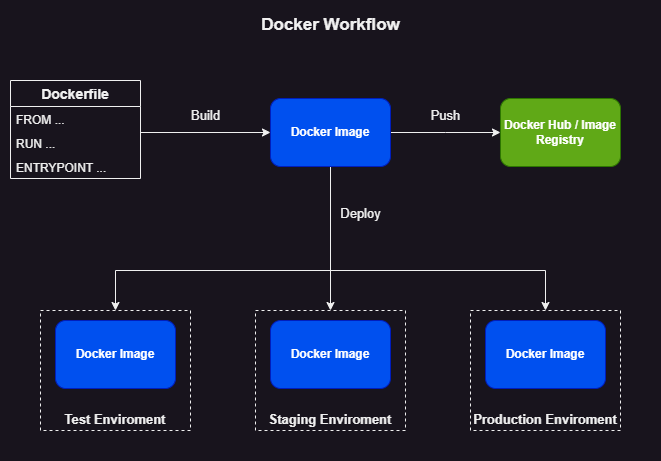
\includegraphics[scale=0.6]{docker_wf.png}
    \centering
    \caption{Docker Workflow}
    \label{fig:docker_wf}
\end{figure}

\section{Prometheus}
Prometheus is an open-source monitoring and alerting toolkit designed to provide flexible, reliable, and robust monitoring for any type of numerical data. It is considered a foundational tool for observability and a key component of modern monitoring stacks. Prometheus excels in collecting, storing, and querying time-series metrics, making it an ideal choice for monitoring infrastructure, applications, and containerized environments.

Prometheus collects and stores metrics as time-series data. Every metric is stored alongside a timestamp, allowing users to track and analyze changes over time. This feature is invaluable for identifying trends, diagnosing performance bottlenecks, and understanding long-term system behavior. Prometheus operates using a pull-based model, periodically scraping selected targets for metrics. This model ensures efficiency by fetching only the required data and enhances security by not requiring external systems to push data directly into Prometheus.

Metrics from various sources are exposed through Exporters, which transform raw data into a Prometheus-readable format. Prometheus includes a large ecosystem of pre-built exporters for common targets such as hardware systems, databases, and cloud platforms. Additionally, creating custom exporters is straightforward, making Prometheus highly adaptable to diverse use cases.

For retrieving, filtering, and manipulating time-series data, Prometheus Query Language (PromQL) is used. PromQL allows users to extract meaningful insights, create advanced visualizations, and define custom alerting rules. Prometheus also integrates seamlessly with Alertmanager, a companion tool for managing alerts. Users can define alerting rules based on PromQL expressions to trigger notifications when specific conditions, such as threshold breaches or anomalies, are met. Alertmanager routes these alerts to appropriate channels, such as email, Slack, or webhooks.

For short-lived jobs that may terminate before Prometheus can scrape their metrics, the PushGateway provides a solution. This intermediary gateway allows these jobs to push metrics temporarily, ensuring no data loss. Prometheus also supports Service Discovery, enabling automatic detection of scrape targets in dynamic environments like Kubernetes. This eliminates the need for manual configuration, making it ideal for large-scale, constantly changing systems.

Prometheus employs a highly optimized, custom-built database for storing time-series data. This database supports fine-grained retention policies, allowing users to define which metrics to retain and for how long, thereby optimizing storage usage. Prometheus further enhances usability with its ability to label metrics using key-value pairs. These labels provide additional context and facilitate filtering and aggregation, enabling multidimensional analysis of metrics.

Although Prometheus offers basic visualization capabilities, it integrates natively with Grafana, the industry-leading visualization platform. This integration allows users to build interactive, feature-rich dashboards. While Prometheus is optimized for metrics collection, it is not suitable for other types of data, such as logs. To complement Prometheus, tools like Loki are often used to handle log data, creating a comprehensive observability stack.\cite{Jani2024-mg,Pragathi2024-fa}



\section{Grafana}
Usually, when utilizing Prometheus to gather metrics, Grafana is employed as the visualization tool of choice. Grafana is an open-source platform for monitoring and observability, designed to enable users to visualize, query, and analyze data from an extensive range of data sources. By transforming raw metrics into actionable insights, Grafana facilitates the creation of complex, interactive dashboards, making it an essential component of most modern monitoring and observability implementations.

These dashboards are highly customizable, combining a diverse variety of visualizations, such as line graphs, heatmaps, gauges, tables, and single-stat panels. This flexibility allows teams to represent various types of information, including historical data, real-time system statuses, and long-term trends, in a visually appealing and intuitive manner.

Grafana supports integration with a broad array of data sources, including Prometheus, Loki, PostgreSQL, MySQL, and cloud services. Its ability to query multiple sources simultaneously enables advanced, multifaceted analyses, where data from disparate systems can be combined and manipulated for deeper insights.

Grafana also has support for variable creation, which allows users to dynamically assign values from the sourced data. This capability enables the construction of dynamic dashboards with parameterized views that adapt to different environments, datasets, or conditions without requiring additional customization. Such dynamic behavior unlocks templating, where reusable dashboards can be developed, significantly enhancing efficiency and consistency across monitoring setups.

Grafana excels at centralizing observability, providing a unified view of the health and performance of systems, services, and applications. Its real-time visualizations empower teams to detect and address issues as they emerge, enabling faster response times and minimizing downtime.

At the same time, the ability to chart and analyze historical data enables the identification of recurring trends and the prediction of potential problems, thus allowing the implementation of proactive measures to mitigate risks.

Lastly, Grafana offers alerting capabilities, same as Prometheus with Alertmanager, that can push notifications on various channels when a set of conditions is met\cite{grafana, promandgraf}.

\begin{figure}[!h]
    \graphicspath{ {./diagrams/} }
    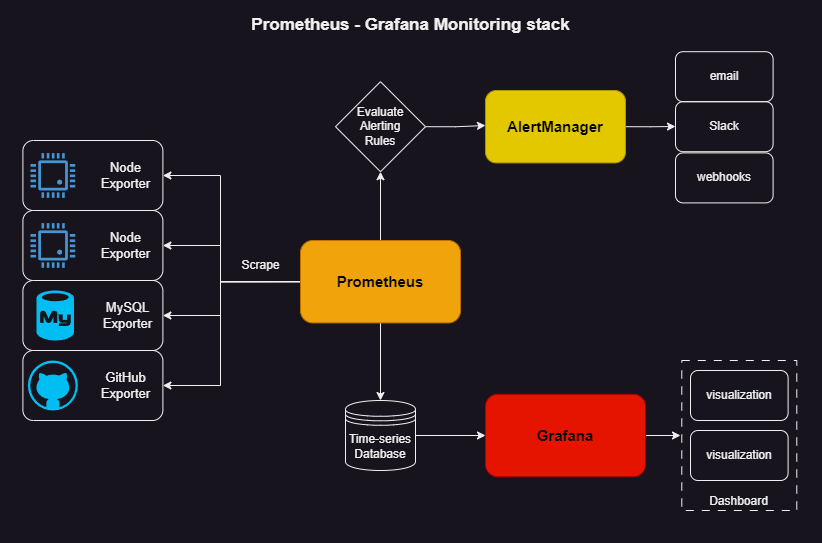
\includegraphics[scale=0.55]{prom-graf.png}
    \centering
    \caption{Prometheus-Grafana Monitoring stack}
    \label{fig:prom_graf}
\end{figure}

\section{Message Queuing Telemetry Transport (MQTT)}
Message Queuing Telemetry Transport (MQTT) is a lightweight, publish/subscribe model messaging protocol specifically designed for devices with limited computational resources and unreliable, low-bandwidth networks. Its efficiency and reliability make it a standard choice for IoT device communication and similar constrained environments.

At its core, MQTT operates using the publish/subscribe model, a decoupled communication architecture where publishers (senders) and subscribers (receivers) exchange messages through a central broker. The MQTT broker serves as the backend system responsible for managing message coordination between clients. Its key responsibilities include receiving and filtering messages, identifying clients subscribed to specific topics, and forwarding messages to those subscribers. Popular MQTT brokers are EMQX, HiveMQ and Mosquitto. Mosquitto was preferred in this implementation for it's lightweight nature, which fits well in a microservice approach.

In typical communication, MQTT clients (which can act as publishers, subscribers, or both) establish a connection with the broker using an MQTT connection. The broker confirms the connection, ensuring both entities are ready to exchange messages. MQTT requires a TCP/IP stack on both clients and brokers for communication, and clients never connect directly with each other but only with the broker. Once connected, the client can either publish messages, subscribe to specific messages, or do both. The broker filters incoming messages using topics, which are structured hierarchically, similar to folder directories in a filesystem. The broker only sends messages to subscribers from the topics they have explicitly subscribed to.

The MQTT protocol is widely regarded as a standard for IoT data transmission and for good reason. Firstly, it requires minimal hardware resources, so it can even be used by small battery-powered microcontrollers. MQTT control messages and MQTT message headers are quite small, reducing network overhead and ensuring efficient use of bandwidth. MQTT has build-in features like quick device reconnections and quality-of-service (QoS) levels, which ensure reliable message delivery even on the unreliable, low-bandwidth and high latency cellular networks IoT devices usually operate on. The decouple nature of MQTT, combined with the low bandwidth requirements allows it to easily handle large number of clients, making it very scalable. 

Despite its many strengths, MQTT does have a few limitations. The broker acts as the central node, and subsequently as a single point of failure, so any disruption or failure of the broker results in a complete communication breakdown. This risk can be mitigated through high-availability setups. Also the maximum payload is 256MB and large payloads can impact performance but in an IoT scenario. However, such large payloads are uncommon. Lastly, MQTT lacks native encryption but modern authentication protocols such as OAuth and TLS can be easily integrated\cite{mqtt}.

\begin{figure}[!h]
    \graphicspath{ {./diagrams/} }
    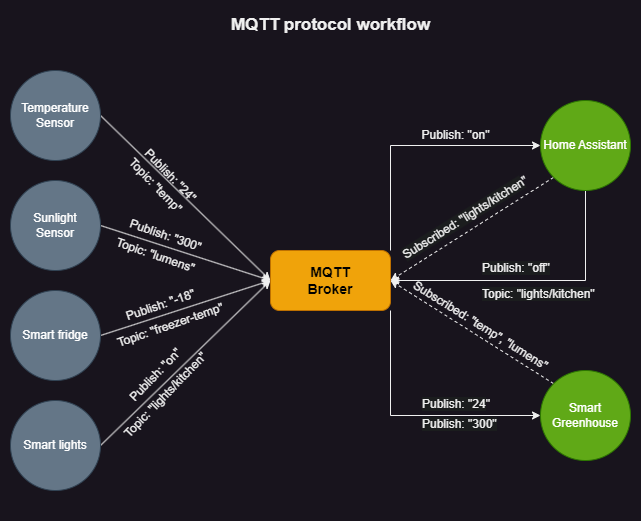
\includegraphics[scale=0.7]{mqtt.png}
    \centering
    \caption{MQTT protocol workflow}
    \label{fig:mqtt}
\end{figure}
 

% Next Chapters
% .............
% .............

%**************************%
%    END OF MAIN THESIS    %
%**************************%

% bibliography
\bibliographystyle{unsrt}
\bibliography{extra/bibliography.bib}
\clearemptydoublepage

% Last Page
\pagestyle{empty}

\vspace*{\fill}
\noindent \hspace{2cm} \rule{12.7cm}{0.4pt}\\
\vspace{-1.7em}
\begin{flushleft}
	\hspace*{30mm}University of Patras, Polytechnic School\\
	\hspace*{30mm}Department of Electrical Engineering \& Computer Technology\\
	\hspace*{30mm}{\nomme}\\
	\hspace*{30mm}© \monthyear \ -- All Rights Reserved\\
\end{flushleft}
\vspace{-1.2em}
\noindent \hspace{2cm} \rule{12.7cm}{0.4pt}

\end{document}